% ===== STEP 2: Define Search Strategy =====
% This section covers:
% - Search strategy development
% - Documentation of search process

\tikzstyle{my-box}=[
    rectangle,
    draw=hidden-black,
    rounded corners,
    text opacity=1,
    minimum height=1.5em,
    minimum width=5em,
    inner sep=2pt,
    align=center,
    fill opacity=.5,
    % line width=0.8pt,
]
\tikzstyle{leaf}=[
    my-box, 
    minimum height=1.5em,
    % fill=hidden-orange!60, 
    fill=hidden-blue!90, 
    text=black,
    align=left,
    font=\normalsize,
    % font=\scriptsize,
    inner xsep=2pt,
    inner ysep=4pt,
    % line width=0.8pt,
]
\begin{figure*}[th!]
    \vspace{-2mm}
    \centering
    \resizebox{\textwidth}{!}{
        \begin{forest}
            forked edges,
            for tree={
                grow=east,
                reversed=true,
                anchor=base west,
                parent anchor=east,
                child anchor=west,
                base=left,
                font=\large,
                rectangle,
                draw=hidden-black,
                rounded corners,
                align=left,
                minimum width=4em,
                edge+={darkgray, line width=1pt},
                s sep=3pt,
                inner xsep=2pt,
                inner ysep=3pt,
                line width=0.8pt,
                ver/.style={rotate=90, child anchor=north, parent anchor=south, anchor=center},
            },
            where level=1{text width=10.2em,font=\normalsize,}{},
            where level=2{text width=8.5em,font=\normalsize,}{},
            where level=3{text width=10.5em,font=\normalsize,}{},
            where level=4{text width=12em,font=\normalsize,}{},
            [
                Deep Learning, ver
                [
                    GPU Programming (\S \ref{sec:task})
                    [
                        Core Libraries
                        [
                            Linear Algebra
                            [
                                \eg cuBLAS (NVIDIA)~\cite{noauthor_cublas_nodate}{,}
                                rocBLAS (AMD)~\cite{noauthor_rocmrocblas_2025}{,}
                                oneMKL (Intel)~\cite{noauthor_uxlfoundationonemath_2025}
                                , leaf, text width=32em
                            ]
                        ]
                        [
                            Deep Learning Primitives
                            [
                                \eg cuDNN (NVIDIA)~\cite{chetlur_cudnn_2014}{,}
                                MIOpen (AMD)~\cite{noauthor_rocmmiopen_2025}{,}
                                oneDNN (Intel)~\cite{onednn_contributors_oneapi_2025}
                                , leaf, text width=32em
                            ]
                        ]
                        [
                            Communication
                            [
                                \eg NCCL (NVIDIA)~\cite{noauthor_nvidianccl_2025}{,}
                                RCCL (AMD)~\cite{noauthor_rocmrccl_2025}{,}
                                oneCCL (Intel)~\cite{noauthor_uxlfoundationoneccl_2025}
                                , leaf, text width=32em
                            ]
                        ]
                    ]
                    [
                        Programming \\ Frameworks
                        [
                            Cross-Platform APIs
                            [
                                \eg OpenCL~\cite{noauthor_khronosgroupopencl-sdk_2025}{,}
                                SYCL~\cite{noauthor_khronosgroupsycl-docs_2025}{,}
                                Kokkos~\cite{trott_kokkos_2022}
                                , leaf, text width=32em
                            ]
                        ]
                        [
                            Vendor-Specific
                            [
                                \eg HIP~\cite{noauthor_rocmhip_2025}{,}
                                CUTLASS~\cite{thakkar_cutlass_2023}
                                , leaf, text width=32em
                            ]
                        ]
                    ]
                    [
                        Language Bindings
                        [
                            Julia Packages
                            [
                                \eg CUDA.jl~\cite{noauthor_juliagpucudajl_2025}{,}
                                AMDGPU.jl~\cite{noauthor_juliagpuamdgpujl_2025}{,}
                                oneAPI.jl~\cite{besard_oneapijl_2022}
                                , leaf, text width=32em
                            ]
                        ]
                        [
                            Python Packages 
                            [
                                \eg CuPy~\cite{okuta_cupy_2017}{,}
                                Numba~\cite{noauthor_numbanumba_2025}
                                , leaf, text width=32em
                            ]
                        ]
                    ]
                    [
                        Learning Resources
                        [
                            Official Tutorials
                            [
                                \eg NVIDIA-Samples~\cite{noauthor_nvidiacuda-samples_2025}{,}
                                AMD-Lab-Notes~\cite{noauthor_amdamd-lab-notes_2025}{,}
                                Intel-Compute~\cite{noauthor_intelcompute-samples_2025}
                                , leaf, text width=32em
                            ]
                        ]
                        Learning Resources
                        [
                            Literature Reviews
                            [
                                \eg Large Scale Deep Learning~\cite{nguyen_machine_2019}{,}
                                , leaf, text width=32em
                            ]
                        ]
                    ]
                ]
                [
                    Distributed Deep \\ Learning (\S \ref{sec:task})
                    [
                        Cloud Solutions
                        [
                            Cloud Platforms
                            [
                                \eg SageMaker~\cite{noauthor_amazon_nodate}{,}
                                BytePS~\cite{jiang_unified_nodate}{,}
                                AzureML~\cite{sdgilley_azure_nodate}{,}
                                Vertex AI~\cite{noauthor_vertex_nodate}
                                , leaf, text width=32em
                            ]
                        ]
                    ]
                    [
                        Framework-Specific
                        [
                            Core Frameworks
                            [
                                \eg PyTorch~\cite{li_pytorch_2020}{,}
                                TensorFlow~\cite{abadi_tensorflow_2016}{,}
                                MXNet~\cite{chen_mxnet_2015}{,}
                                JAX~\cite{frostig_compiling_nodate}
                                , leaf, text width=32em
                            ]
                        ]
                        [
                            Extensions
                            [
                                \eg Transformers~\cite{wolf_huggingfaces_2020}{,}
                                Lightning~\cite{noauthor_overview_nodate}
                                , leaf, text width=32em
                            ]
                        ]
                    ]
                    [
                        General-Purpose
                        [
                            Universal Frameworks
                            [
                                \eg Colossal-AI~\cite{li_colossal-ai_2023}{,}
                                Ray~\cite{moritz_ray_2018}{,}
                                Horovod~\cite{sergeev_horovod_2018}
                                , leaf, text width=32em
                            ]
                        ]
                    ]
                    [
                        Specialized Tools
                        [
                            Large Model Training
                            [
                                \eg Megatron-LM~\cite{shoeybi_megatron-lm_2020}{,}
                                GPipe~\cite{huang_gpipe_2019}{,}
                                DeepSpeed~\cite{rasley_deepspeed_2020}{,}
                                FairScale~\cite{noauthor_fairscale_nodate}
                                , leaf, text width=32em
                            ]
                        ]
                        [
                            Research
                            [
                                \eg GShard~\cite{lepikhin_gshard_2020}
                                , leaf, text width=32em
                            ]
                        ]
                    ]
                    [
                        [
                            Distributed
                            [
                                \eg Pylearn2~\cite{Goodfellow.EtAl_2013}{,} Torch7~\cite{Collobert.EtAl_}{,} Caffe~\cite{Jia.EtAl_2014a}{,} Cuda-Convnet~\cite{krizhevsky_imagenet_2012}
                                , leaf, text width=32em
                            ]
                        ]
                    ]
                    [
                        Learning Resources
                        [
                            Official Tutorials
                            [
                                \eg Pytorch DDP~\cite{noauthor_examplesdistributedddpreadmemd_nodate}
                                , leaf, text width=32em
                            ]
                        ]
                        Learning Resources
                        [
                            Literature Reviews
                            [
                                \eg Distributed Deep Learning Surveys~\cite{dehghani_distributed_2023}{,}
                                \cite{chahal_hitchhikers_2018}{,}
                                \cite{berloco_systematic_2022}
                                , leaf, text width=32em
                            ]
                        ]
                    ]
                ]
            ]
        \end{forest}
    }
    \vspace{-4mm}
    \caption{Taxonomy of deep learning for mathematical reasoning. The associated tasks are elaborated in \S \ref{sec:task}, with a comprehensive dataset list found in \S \ref{sec:dataset}. Deep learning methods are further discussed in \S \ref{sec:network}, \S \ref{sec:pretrain}, and \S \ref{sec:icl}.}
    \label{fig:taxonomy}
    \vspace{-3mm}
\end{figure*}

\begin{figure*}[th]
	\centering
	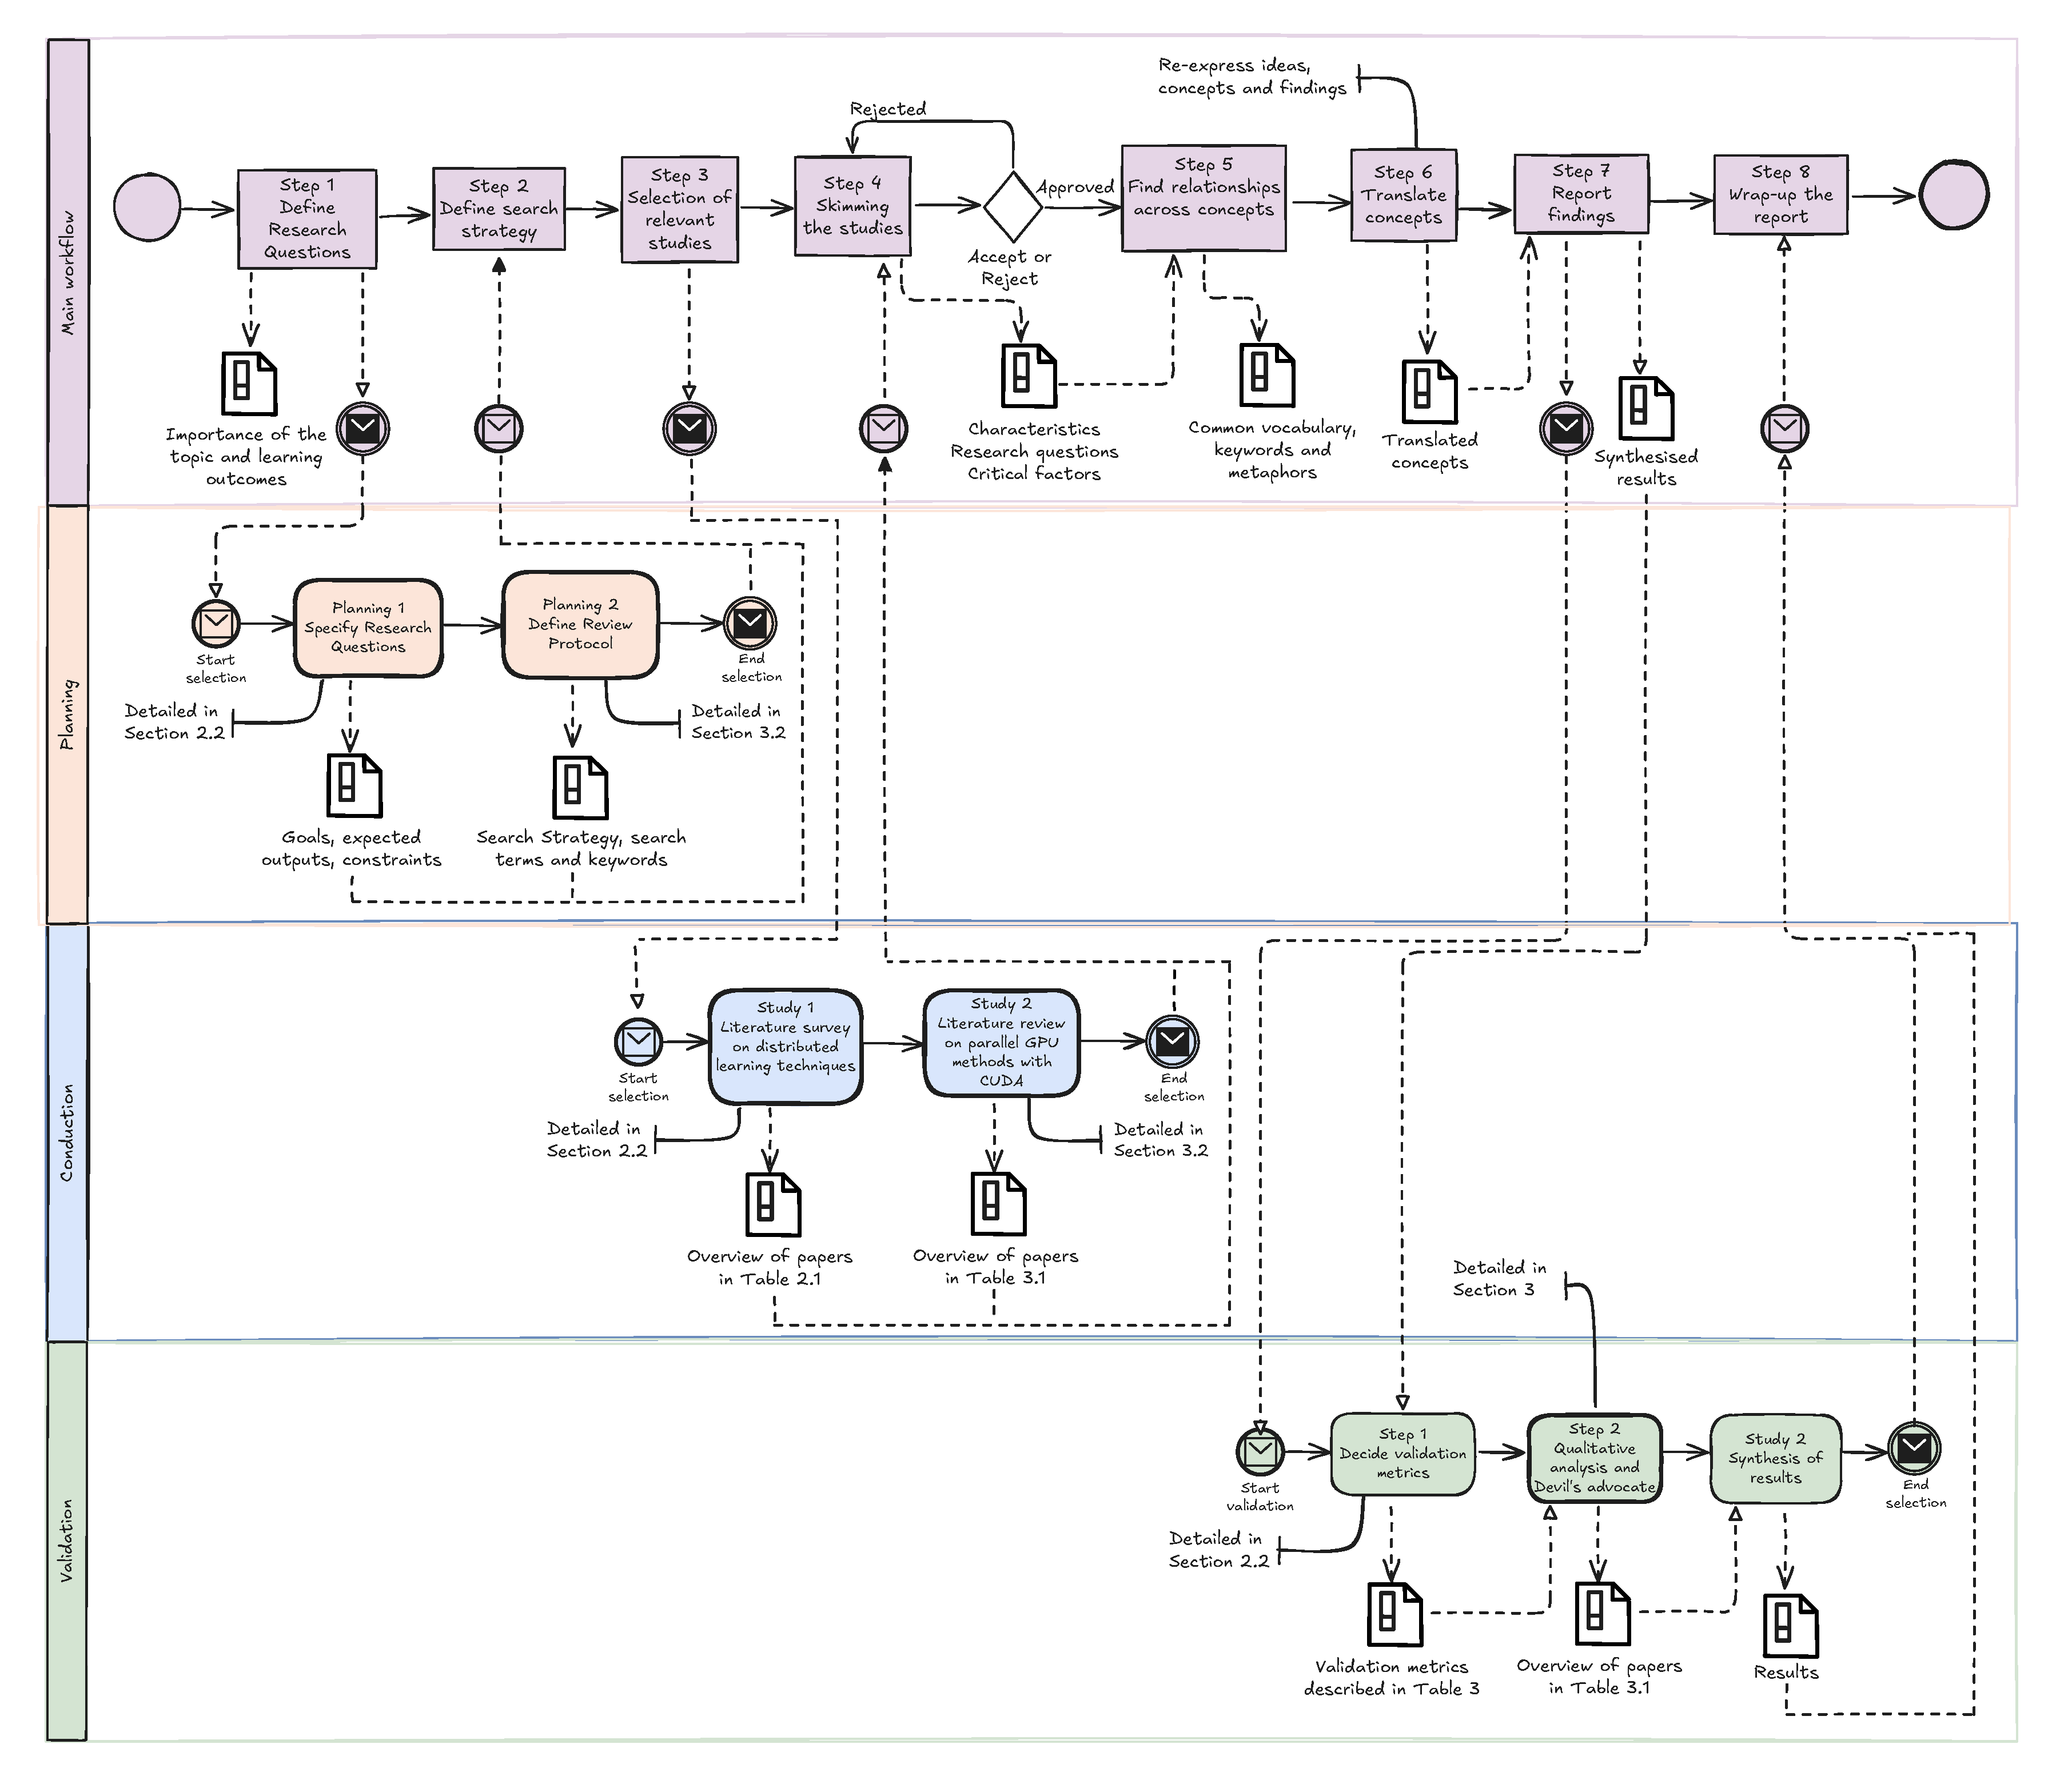
\includegraphics[width=\linewidth]{figures/workflow2}
	\caption{Systematic review workflow showing the main steps, documentation artifacts, and validation processes.
		The workflow is divided into three main phases: main workflow (top), studies selection (middle), and
		validation (bottom). Dashed lines indicate documentation and communication flows. Adapted from \cite{dos_santos_sustainable_2024}.}
	\label{fig:workflow}
\end{figure*}

\section{Related Work}
\label{sec:related_work}

\TODO{Reference the related work on survying the present methods both in DDL and CUDA}

For documenting the review process, this study follows primarily the guidelines laid out in
\cite{keele_systematic_2007}, however advice for conducting the review is synthesized from a wider
range of related articles
\cite{brereton_lessons_2007-1,kitchenham_procedures_nodate,budgen_reporting_2018,dos_santos_sustainable_2024}.

\textbf{Limitations of existing work.}
Our study differs from previous surveys in a few different aspects. First, concerning the DNN part,
related work focuses on techniques and algorithms for training models across multiple machines
\cite{dehghani_distributed_2023, chahal_hitchhikers_2018, berloco_systematic_2022}, where themes
such as data and model parallelization techniques and communication protocols are explored. As a
result, existing literature tackles architectural patterns and design choices, none focusing
explicitly on providing a broad review of the available frameworks. Secondly, although existing
repositories do provide examples on how to use the CUDA library
\cite{noauthor_nvidiacuda-samples_2025}, as well as DDP
\cite{noauthor_examplesdistributedddpreadmemd_nodate}, none provide end-to-end implementations that
would allow the community to build upon. This study aims to answer both of these concerns.

Another relevant article which aims to provide an overview of massive parallel frameworks available
for deep learning is \cite{nguyen_machine_2019}. It describes specialized tools for hardware
accelerators (GPUs, FPGAs, TPUs), however does not focus on auxiliary libraries for linear algebra,
numerical computing and GPU communication, gap which this study aims to fill.

Below are summarized some of the key concepts that the rest of this review builds upon:

\begin{itemize}
	\item \textbf{Data Parallelism:}
	      The dataset is divided across multiple nodes, with each node training a complete copy of the
	      model on its portion of data. Gradients from all nodes are then combined to update the model parameters.
	      This approach can be implemented either synchronously (all nodes wait for each other) or asynchronously (nodes work independently).

	\item \textbf{Model Parallelism:}
	      The neural network model itself is divided across different nodes, with each node responsible
	      for computing a specific portion of the model architecture. This strategy is particularly useful
	      when the model is too large to fit on a single machine.

	\item \textbf{Pipeline Parallelism:}
	      The training process is divided into sequential stages, similar to an assembly line,
	      where the output of one stage becomes the input for the next. This allows different parts
	      of the model to train simultaneously while maintaining dependencies.

	\item \textbf{Hybrid Parallelism:}
	      This approach combines multiple parallelization strategies to optimize training efficiency.
	      For example, model parallelism might be used to distribute a large model across GPUs, while
	      data parallelism is applied to each model segment.
\end{itemize}

These approaches can be further enhanced through techniques such as gradient compression, mixed
precision training, and tensor fusion \cite{dehghani_distributed_2023}. The choice of specific
techniques depends on factors including model architecture, available hardware, and training
requirements. For a comprehensive review of these techniques and their implementations, readers are
referred to \cite{chahal_hitchhikers_2018}.

\section{Research method}
\label{sec:protocol}

Multiple studies emphasize that a literature survey should be both transparent and replicable
\cite{keele_systematic_2007, dos_santos_sustainable_2024-1}, as this can ensure that review bias is
minimized. This is a valid concern in general, however especially so in this survey since it is
conducted by only one person. In a broader study, bias would normally be minimized by having
multiple iterations with more than one reviewer involved. In this paper, steps have been taken to
mitigate this problem, nonetheless it is acknowledged that it is not possible to eliminate it
completely. To ensure this, the process is documented, most of the resulting artifacts being
available in the text as well as in the Appendix.

% TODO these are all good but was hoping to minimize the number of citations
% TODO \cite{keele_systematic_2007,brereton_lessons_2007-1,budgen_reporting_2018, dos_santos_sustainable_2024-1},

% Now detail Step 1 content
The process workflow is shown in Figure \ref{fig:workflow} where the key phases are annotated as
follows: Getting Started (M.1, M.2), Planning the Review (M.3, M.4), Conducting the Review (M.5,
M.6), and Reporting the Review (M.7, M.8). M.2 calls an auxiliary process composed of S.1 and S.2
to select the appropriate studies.

\subsection{M.1 -- The need for a survey}
\label{sec:need_for_survey}

\textbf{Importance of the topic.}
Distributed techniques are important in neural networks because they allow models with billions of
parameters to perform a large number of computations in a reasonable amount of time. One of the
pioneering papers in machine learning that made use of GPUs to train neural networks in parallel
(AlexNet \cite{krizhevsky_imagenet_2012}), mentioned that the network took "between five and six days to
train on two GTX 580 3GB GPUs", suggesting that the training time would have taken much longer on a
CPU.

One key property of distributing neural network architectures to a larger number of parameters, is
that one can achieve better generalization and lower error rates even when training on smaller
datasets \cite{kaplan_scaling_2020}. This has applications in many domains, among which natural
language processing, computer vision and speech recognition \cite{noauthor_papers_nodate}.

\textbf{Learning outcomes.}
As a result of conducting the survey I expect the following learning outcomes: generally get accustomed
with the frameworks that enable distributed training of neural networks and gain practical experience
conducting experiments with CUDA and Pytorch DDP.

\subsection{M.2 -- Getting started}
\label{sec:research_questions}
The main goal is to analyze parallelization frameworks in DNNs and GPU programming. This entails two distinct
constraints: (i) consider only frameworks that introduce GPU programming and DNN frameworks and (ii) include
only primary studies.

\subsection{M.3 -- Selection of Relevant Studies}
This step identified and selected studies from both areas (GPU programming in S.1 and DNN
frameworks). I collected studies of the state of the art of both GPU programming (in Step S.1) and
DNN frameworks (in Step S.2).

\subsubsection{S.1 -- Literature Survey on DNN libraries}
\paragraph{S.1.1 -- Problem definition.}
In order to identify relevant studies, I conducted a secondary study\footnote{A secondary study
	synthesizes primary papers to provide a comprehensive overview. This contrasts with tertiary
	studies which analyze secondary studies.}. This decision was made in the problem definition step
(S.1.1 in Figure \ref{fig:workflow-study-cuda}). To ensure a methodical approach, this section
defines a research protocol which formally defines the key attributes of the search process. This
basically entails expanding on the research questions and search strategy.

\begin{figure*}[th]
	\centering
	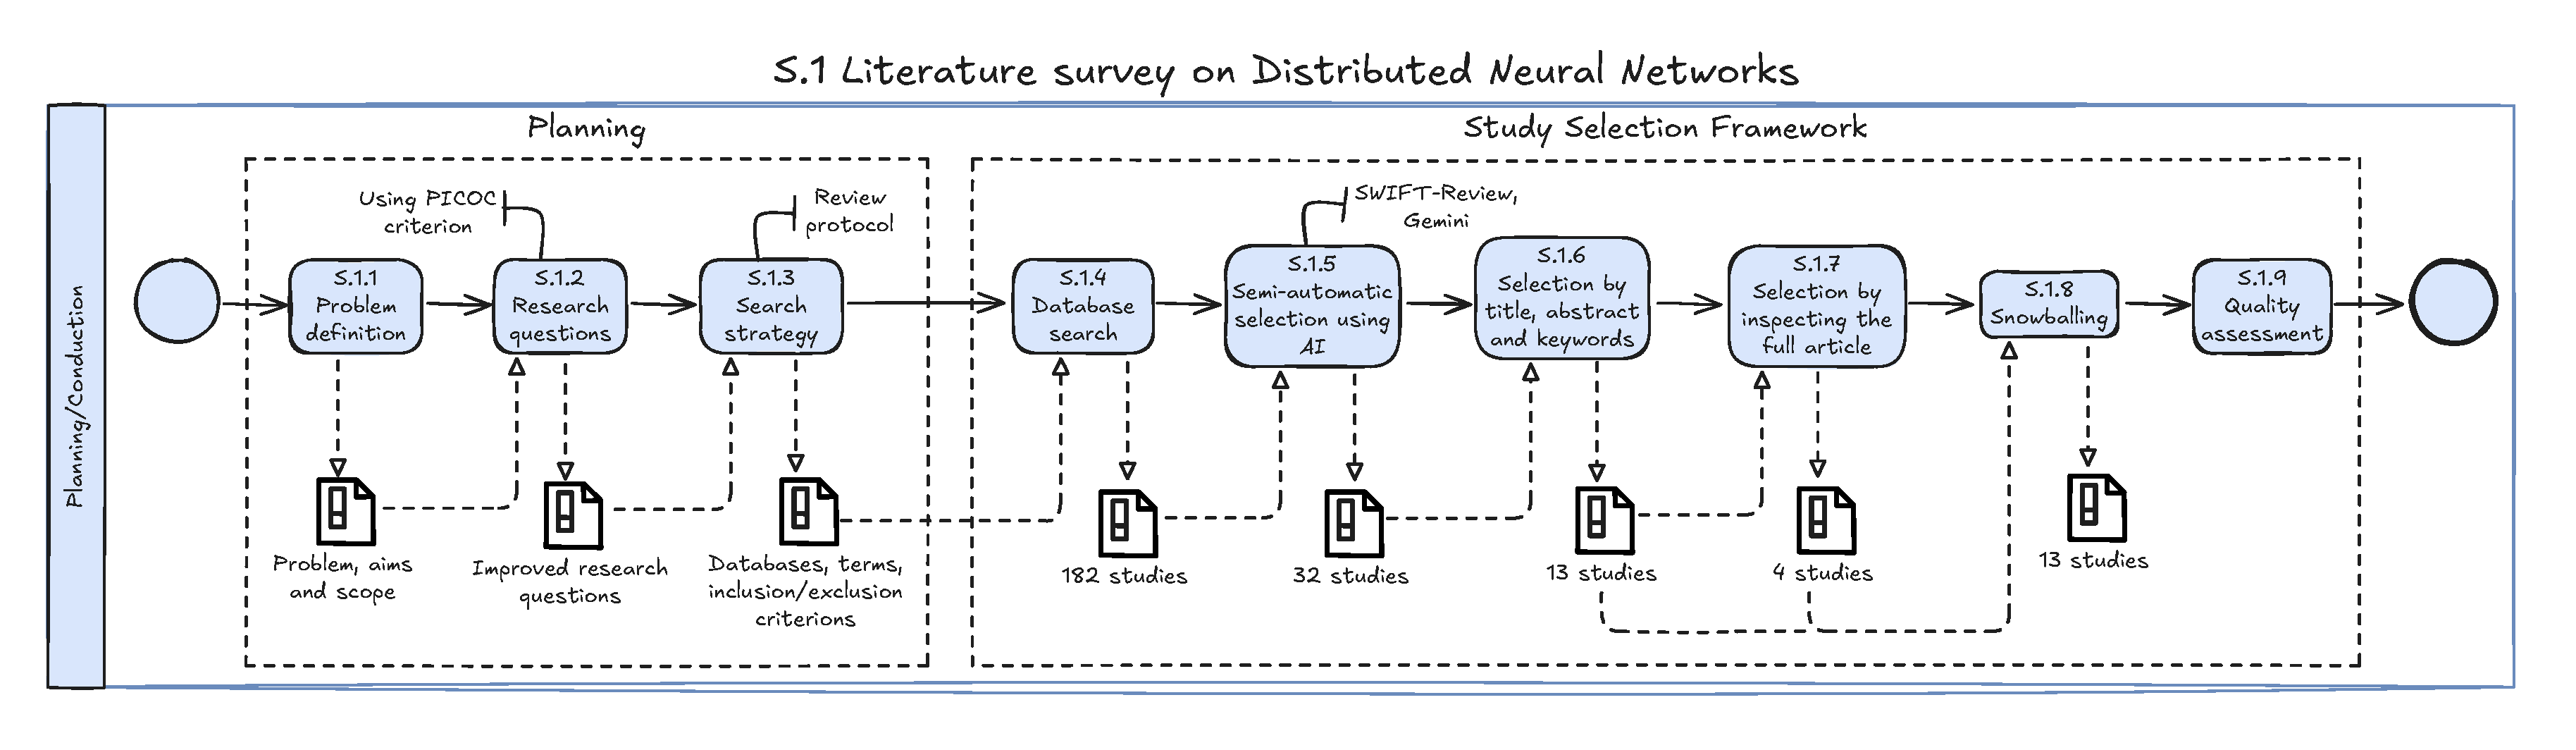
\includegraphics[width=\linewidth]{figures/survey-dnn.pdf}
	\caption{The diagram suggests the key steps for finding papers related to the CUDA programming survey. The phases
		include planning the review (aims, research questions, search strategy) and conducting the review (study selection phase). The research questions
		were transformed according to the PICOC (Population, Intervention, Comparison, Outcome, Context) criterion suggested by \cite{keele_systematic_2007}.}.
	\label{fig:workflow-study-cuda}
\end{figure*}

\paragraph{S.1.2 -- Research questions.}
After an initial literature review, the research questions (RQ) defined in Section
\ref{sec:initial_research_questions} are refined using the guidelines defined in
\cite{kitchenham_evidence-based_2015} and \cite{keele_systematic_2007}. Specifically, the PICOC
(Population, Intervention, Comparison, Outcome, Context) criterion is used to transform the
questions into a format that ensures them to be specific, measurable and well-defined. The
questions below are ordered based on their priority in the survey:

% TODO: remove this
% \begin{itemize}
% 	\item \textbf{RQ\textsubscript{1}} What are the most common frameworks currently available for 
% 		  GPU programming with CUDA, and how do their usability compare?
% 		  % NOTE implementing distributed deep learning, and how does their usability compare?
% 	      % NOTE \cite{berloco_systematic_2022, ben-nun_demystifying_2020, langer_distributed_2020}?
% 	      % NOTE \item How do parameter update strategies impact distributed deep learning systems (e.g., Parameter Server and decentralised approaches) \cite{ben-nun_demystifying_2020,berloco_systematic_2022,langer_distributed_2020}?
% 	\item How is stochastic gradient descent (SGD) computed in distributed environments
% 	      \cite{berloco_systematic_2022,ben-nun_demystifying_2020,langer_distributed_2020,verbraeken_survey_2021}? % NOTE and what are the associated challenges 
% 	\item What are the key frameworks currently available for implementing DDL, and how do their features 
% 	      compare \cite{berloco_systematic_2022}?
%  	\item In what ways are the techniques used in DDL also useful in GPU parallelization?
% \end{itemize}

% TODO: \TODO{RQ1: ease of learning, ease of use and documentation compare?}
\label{sec:research_questions_refined}
\begin{itemize}
	\item \textbf{RQ\textsubscript{1}:} In the field of Deep Learning, what are the most commonly cited
	      frameworks for distributed training of neural networks across clusters, and how do their respective communities vary in size? \\
	      \textit{Rationale:} By identifying the most common frameworks, we can trace the years in which they were published
	      and form a unified timeline of the evolution of the field with respect to the related GPU programming advancements.

	      % NOTE Razvan I am conducting a literature review in the field of deep learning, specifically focusing on distributed training of 
	      % NOTE neural networks across clusters. I need to identify the most commonly cited frameworks used for this purpose.
	\item \textbf{RQ\textsubscript{2}:} What practical applications of these technologies have been reported in the literature? \\
	      \textit{Rationale:} This can yield hands-on experience on the topic which is helpful for practical applications.

	\item \textbf{RQ\textsubscript{3}:} What are the overlaps in data/model optimization strategies used in DDL and GPU parallelization? \\
	      \textit{Rationale:} By identifying the overlaps, this can lead to a more comprehensive understanding of the field.
\end{itemize}

The questions play a key role in guiding the search strategy, data extraction process and results
synthesis phase.

\paragraph{S.1.3 -- Search Strategy.}
The search strategy represents represents a systematic approach for identifying relevant studies
that adequately answer the research questions.

\textbf{Databases.}
The process involves a manual search of three citation databases --
\href{https://www.scopus.com/}{Scopus}, \href{https://www.semanticscholar.org/}{Semantic Scholar}
and \href{https://arxiv.org/}{arXiv}\footnote{Other relevant databases that could have been used
	include: \href{https://ieeexplore.ieee.org/}{IEEE Xplore}, \href{https://dl.acm.org/}{ACM Digital
		Library} and \href{https://www.sciencedirect.com/}{Science Direct}.} -- that include conference
proceedings and journal papers, considering three metadata fields (title, abstract, and keywords).

\textbf{Inclusion/Exclusion Criteria.}
There were defined three inclusion criteria (IC) and three exclusion criteria (EC). In particular, I
decided to select only primary studies, however secondary studies were mentioned in Section
\ref{sec:related_work}. The identification of secondary studies was useful since the selected
studies synthesize evidence and can make it possible to access primary studies:

\begin{itemize}
	\item \textbf{IC\textsubscript{1}}: Study is a primary study.
	\item \textbf{IC\textsubscript{2}}: Study addresses distributed frameworks in DL.
	\item \textbf{IC\textsubscript{3}}: Study introduces a library or a framework. \\
	\item \textbf{EC\textsubscript{1}}: Study does not discuss implementation details.
	\item \textbf{EC\textsubscript{2}}: Study is not a primary study.
	\item \textbf{EC\textsubscript{3}}: Study is not written in English.
\end{itemize}

\textbf{Search terms.}
In Step S.1.3, I inquired about the literature using the following search string:
\begin{quote}
	\textit{( "machine learning" OR "deep learning" )
		AND
		( "Data parallelism" OR "model parallelism")
		AND
		( "framework" OR "implementation" )}
\end{quote}

The details and justification to define this search string can be found in the supplementary
material in Section \ref{sec:search_strategy}. \TODO{...}

\paragraph{Publication year criteria.}
For the DDL task, papers were considered between $\yearstartddl$-$\yearendddl$. The start year
($\yearstartddl$) was chosen as at this point there was a shift towards resource conservation,
which resulted in a focus on concurrency within mini-batches \cite{ben-nun_demystifying_2020}. This
is the year by which the effectiveness of deep learning algorithms was more widely recognized and
more research was published that focused on scalability.

\paragraph{S1.4 - S1.5 -- Semi-Automatic selection.}
After an initial database search (Step S1.4), 182 studies were retrieved. Subsequently, as part of
S.1.5, two methods were applied for reducing the number of studies to a more manageable set. Below,
I describe each approach, including my evaluation regarding their effectiveness.

\textbf{Swift-Review.}
As suggest in \cite{bolanos_artificial_2024},
I applied Swift-Review \cite{Howard2016SWIFTReviewAT}, a machine learning classifier to filter out
irrelevant studies (Step S.1.5). The technique is semi-automatic
with a focus on screening and extraction of relevant information. Prior to initiating the classification,
I had to manually identify 10 positive and 10 negative examples. These
acted as input seed samples for the classifier, which helped pinpoint other useful material. Then
the classifier identified other relevant papers by screening the title, abstract and keywords of
each study. All papers with a confidence score above 0.5 are selected.

\textbf{Classification using Gemini.}
The downside of the previous approach is that it still involves a lot of work to manually identify key
studies. To address this, \cite{bolanos_artificial_2024} suggests many emerging tools that use Large Language Models (LLMs)
to automatically classify relevant material. However, in my experience, none are particularly effective
at handling a large corpus of text due to the context window being relatively small. As a result, I decided
to use Gemini \cite{team_gemini_2024} to classify the studies, which is a particularly strong choice due to its massive
context window (over 2M tokens). The drawback is that Gemini does not provide citations when using the web interface
\cite{noauthor_gemini_nodate}. However, NotebookLM \cite{notebooklm_google_2024} solves the issue by providing references
to portions of the text that are relevant to the query. My approach involved downloading the search results in textual format from the
search engines and then leveraging NotebookLM to classify the studies by utilizing the research questions
defined in Section \ref{sec:research_questions} as a prompt. This was an iterative process that involved
reading the abstracts and keywords of each study to ascertain about the reliability of each response. It is not a perfect process,
however building iteratively over the results and blending together different phases of the review process
(as we shall see in Section \ref{sec:reading-studies}), gives a good baseline for iterative improvement.

\textbf{Results.}
After investigating the results of both approaches, I found that the NotebookLM approach was more
effective at identifying key studies. This is likely due to Gemini being a more powerful
model than the classifier used by Swift-Review. The number of selected studies was 32.

\paragraph{S.1.6 - S.1.8 -- Manual selection.}
In Step S.1.6, a manual inspection over the the title, abstract and keywords was made. This
resulted in a total of 13 studies that appeared to be relevant. After checking their full text,
this number was reduced to 4. I performed backward snowballing \cite{jalali_systematic_2012} by
revisiting the references of the 4 studies, as well as checking available preprint articles and
identified other 8 studies (Step 1.8). Hence, a total of 12 studies (4 + 8) were selected. A
subsequent 5 frameworks were found with no accompanying papers by reviewing the references. All 17
libraries are listed in Table \ref{tab:dnn_papers}.

\begin{table}[h!]
	\centering
	\caption{The Search Engines Used in this Survey}
	\label{tab:databases}
	\begin{tabular}{llllr}
		\hline
		ID    & Tool             & Step  & Results & Filtered \\
		\hline
		1     & Scopus           & S.1.4 & 182     & 4        \\
		2     & Semantic Scholar & S.1.8 & --      & 8        \\
		3     & Proprietary      & S.1.8 & --      & 5        \\
		\hline
		Total &                  &       &         & 17       \\
	\end{tabular}
\end{table}

\paragraph{S.1.9 -- Quality assessment.}
To evaluate the quality of these studies (Step S.1.9), I adapted the quality appraisal instrument
suggested by \cite{zhou_map_2016}, considering 2 main aspects: report and relevance. Regarding
report, I checked whether the studies clearly tackled the problem, research questions and
inclusion/exclusion criteria defined in Steps S.1.1, S.1.2 and S.1.3 respectively. Concerning
relevance, I verified whether the studies presented relevant information to ensure their value for
practitioners and researchers. Finally, all 17 studies identified in the previous steps passed the
quality checks.

\begin{table*}[h!]
	\centering
	\caption{The DNN papers included in the review. 1 (data), 2 (model), 3 (pipeline)}
	\label{tab:dnn_papers}
	\begin{tabular}{llp{8.4cm}lllc}
		\hline
		\small \textbf{\#} & \small \textbf{Ref.}                    & \small \textbf{Title}                                                                                                               & \small \textbf{Type} & \small \textbf{Year} & \small \textbf{Citations} & \small \textbf{Stars}                                                \\[1ex]
		\hline
		\small DNN1        & \small \cite{abadi_tensorflow_2016}     & \small TensorFlow: Large-Scale Machine Learning on Heterogeneous Distributed Systems                                                & \small Data          & \small 2016          & \small 9998               & \small 187k \cite{abadi_tensorflow_2015}                             \\[1ex]
		\small DNN2        & \small \cite{chen_mxnet_2015}           & \small MXNet: A Flexible and Efficient Machine Learning Library for Heterogeneous Distributed Systems                               & \small Hybrid        & \small 2015          & \small 2214               & \small 20.8k \cite{noauthor_apachemxnet_2025}                        \\[1ex]
		\small DNN3        & \small \cite{huang_gpipe_2019}          & \small GPipe: Efficient Training of Giant Neural Networks using Pipeline Parallelism                                                & \small Pipeline      & \small 2018          & \small 1446               & \small 2.8k \cite{noauthor_tensorflowlingvo_2025}                    \\[1ex]
		\small DNN4        & \small \cite{jiang_unified_nodate}      & \small BytePS: A Unified Architecture for Accelerating Distributed DNN Training in Heterogeneous GPU/CPU Clusters                   & \small Data          & \small 2020          & \small 338                & \small 3.7k \cite{noauthor_bytedancebyteps_2025}                     \\[1ex]
		\small DNN5        & \small \cite{lepikhin_gshard_2020}      & \small GShard: Scaling Giant Models with Conditional Computation and Automatic Sharding                                             & \small Model         & \small 2020          & \small 931                & \small 2.8k \cite{noauthor_tensorflowlingvo_2025}                    \\[1ex]
		\small DNN6        & \small \cite{li_pytorch_2020}           & \small PyTorch Distributed: Experiences on Accelerating Data Parallel Training                                                      & \small Hybrid        & \small 2020          & \small 175                & \small 86.1k \cite{noauthor_pytorchpytorch_nodate}                   \\[1ex]
		\small DNN7        & \small \cite{li_colossal-ai_2023}       & \small Colossal AI: A Unified Deep Learning System for Large-Scale Parallel Training                                                & \small Hybrid        & \small 2023          & \small 118                & \small 39k \cite{noauthor_hpcaitechcolossalai_2025}                  \\[1ex]
		\small DNN8        & \small \cite{moritz_ray_2018}           & \small Ray: A distributed Framework for Emerging AI Applications                                                                    & \small Hybrid        & \small 2018          & \small 1108               & \small 35k \cite{noauthor_ray-projectray_2025}                       \\[1ex]
		\small DNN9        & \small \cite{rasley_deepspeed_2020}     & \small DeepSpeed: System Optimizations Enable Training Deep Learning Models with Over 100 Billion Parameters                        & \small Hybrid        & \small 2020          & \small 1059               & \small 36.3k \cite{noauthor_microsoftdeepspeed_2025}                 \\[1ex]
		\small DNN10       & \small \cite{sergeev_horovod_2018}      & \small Horovod: fast and easy distributed deep learning in TensorFlow                                                               & \small Data          & \small 2018          & \small 1152               & \small 14.3k \cite{noauthor_horovodhorovod_2025}                     \\[1ex]
		\small DNN11       & \small \cite{shoeybi_megatron-lm_2020}  & \small Megatron-LM: Training Multi-Billion Parameter Models for Natural Language Processing                                         & \small Hybrid        & \small 2020          & \small 1578               & \small 11.2k \cite{noauthor_nvidiamegatron-lm_2025}                  \\[1ex]
		\small DNN12       & \small \cite{wolf_huggingfaces_2020}    & \small HuggingFace's Transformers: State-of-the-art Natural Language Processing                                                     & \small Data          & \small 2020          & \small 1444               & \small 8.2k \cite{noauthor_huggingfaceaccelerate_2025}               \\[1ex]
		\small DNN13       & \small \cite{noauthor_overview_nodate}  & \small Pytorch Lightning: The lightweight PyTorch wrapper for high-performance AI research. Scale your models, not the boilerplate. & \small Data          & \small 2019          & \small N/A                & \small 28.8k \cite{falcon_pytorch_2019}                              \\[1ex]
		\small DNN14       & \small \cite{noauthor_fairscale_nodate} & \small FairScale:  A general purpose modular PyTorch library for high performance and large scale training                          & \small Hybrid        & \small 2021          & \small N/A                & \small 3.2k \cite{FairScale2021}                                     \\[1ex]
		\small DNN15       & \small \cite{noauthor_amazon_nodate}    & \small Amazon SageMaker Platform                                                                                                    & \small Data          & \small 2017          & \small N/A                & \small 10.3k \cite{noauthor_awsamazon-sagemaker-examples_2025}       \\[1ex]
		\small DNN16       & \small \cite{sdgilley_azure_nodate}     & \small Microsoft AzureML Platform                                                                                                   & \small Data          & \small 2021          & \small N/A                & \small 1.8k \cite{noauthor_azureazureml-examples_2025}               \\[1ex]
		\small DNN17       & \small \cite{noauthor_vertex_nodate}    & \small Google Vertex AI Platform                                                                                                    & \small Data          & \small 2021          & \small N/A                & \small 178 \cite{noauthor_googlecloudplatformvertex-ai-samples_2025} \\[1ex]
		\small DNN18       & \small \cite{frostig_compiling_nodate}  & \small Jax: Compiling machine learning programs via high-level tracing                                                              & \small Hybrid        & \small 2018          & \small N/A                & \small 31k \cite{noauthor_jax-mljax_2025}                            \\[1ex]
		\hline
	\end{tabular}
\end{table*}

\subsubsection{S.2 -- Survey on GPU programming libraries}
\label{sec:gpu-programming-libraries}
This step involved identifying popular frameworks that facilitate programming on the GPU. The
workflow that was followed is shown in Figure \ref{fig:workflow-study-cuda}.

\paragraph{S.2.1 -- Problem definition.}
It was not possible to perform a systematic review in the traditional sense due to the nature of
the available tools. The available libraries are frequently proprietary and are rarely accompanied
by academic papers. Also, the libraries are implementation-focused with documentation and tutorials
being the main source of information. As a result, I had to widen out the type of articles to
include in the review by referencing useful tutorials and key documentation pages.

\paragraph{S.2.2 -- Research Questions.}
The research questions defined in Section \ref{sec:initial_research_questions} were refined using
the PICOC criterion suggested by \cite{keele_systematic_2007}. The following question is relevant:

\begin{itemize}
	\item \textbf{RQ\textsubscript{4}:} In the field of Deep Learning, what are the most frequently cited
	      frameworks for GPU programming using CUDA, and how do their user communities differ in size? \\
	      \textit{Rationale:} By identifying the most common frameworks, we can identify which are the gaps
	      in the literature they cover and which are the most promising areas for future research.
\end{itemize}

Moreover, questions RQ\textsubscript{2} and RQ\textsubscript{3} from Section
\ref{sec:research_questions_refined} are also relevant.

\paragraph{S.2.3 -- Search strategy.}
To find relevant materials (Github repositories, documentation pages and tutorials), the following
tools were used: \href{https://github.com/search/advanced}{Advanced Github Search} and two AI
search engines: DeepSeek Search Engine \cite{noauthor_deepseek_nodate} and Perplexity AI
\cite{noauthor_perplexity_nodate}.

\begin{figure*}[th]
	\centering
	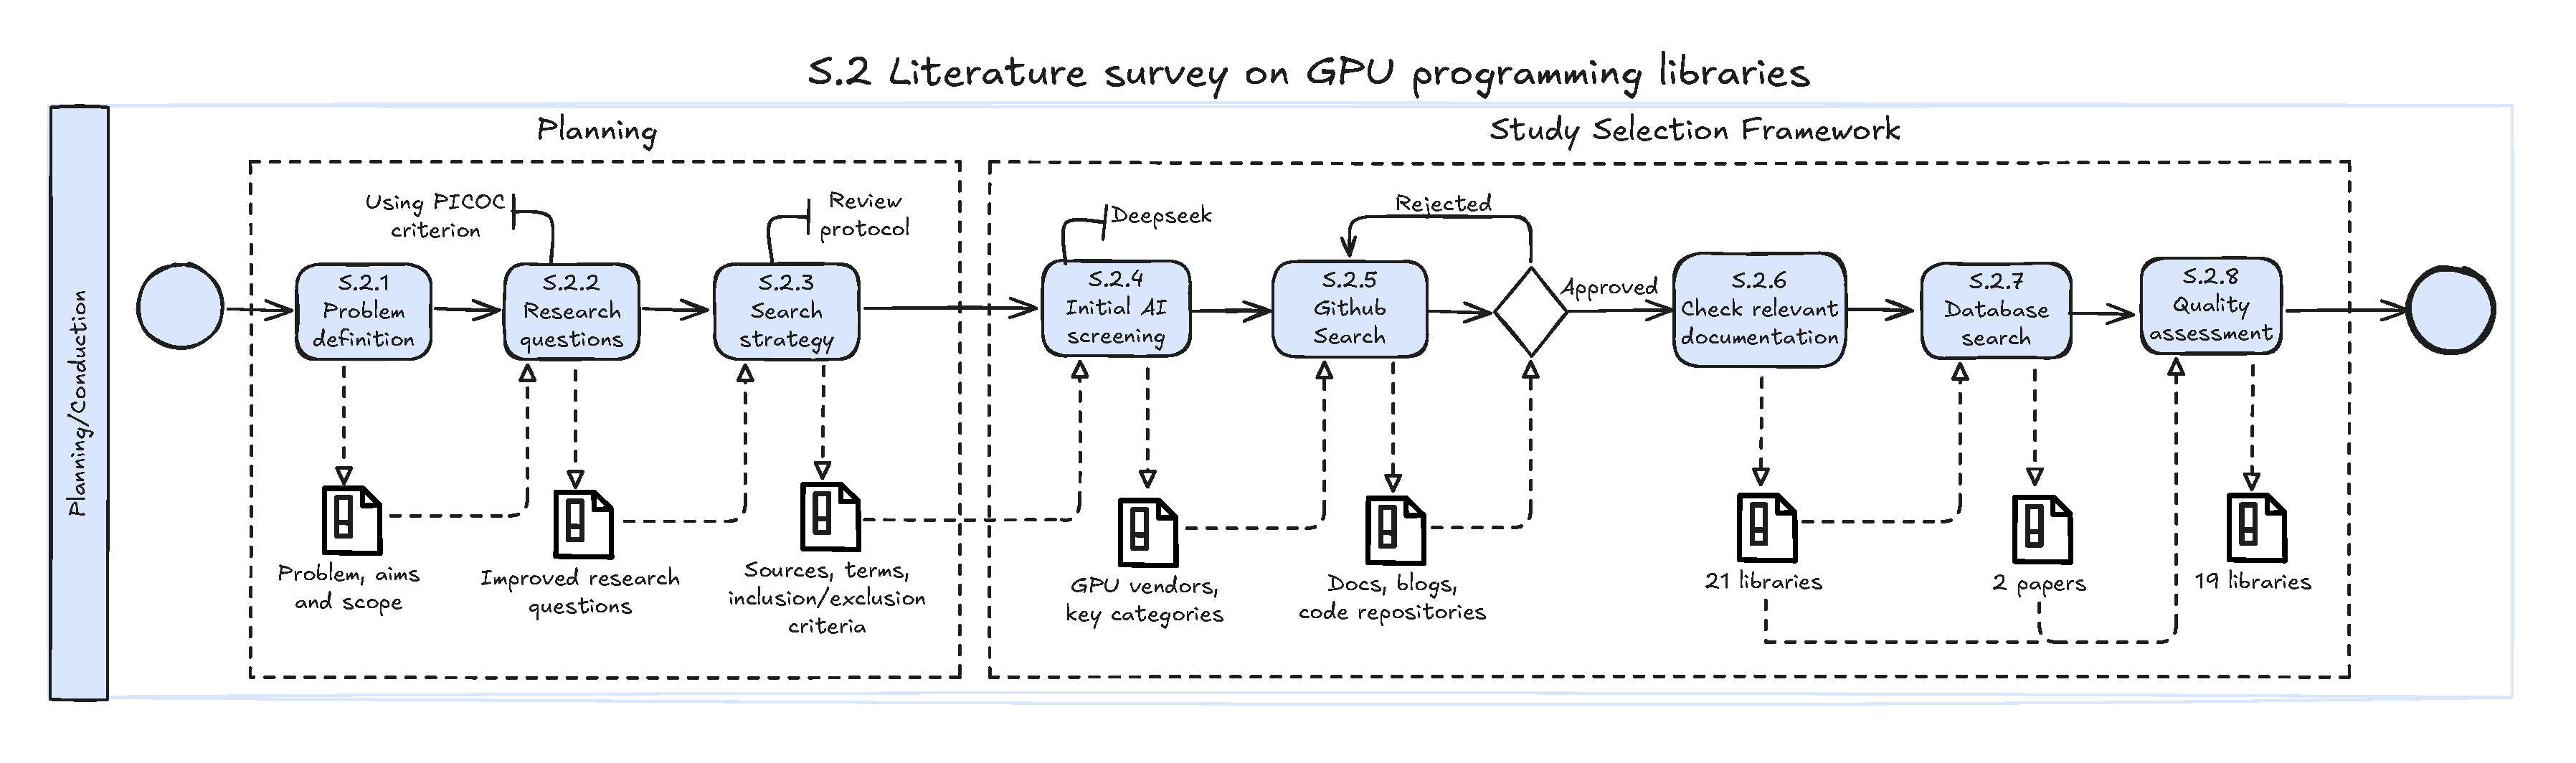
\includegraphics[width=\linewidth]{figures/survey-cuda3.pdf}
	\caption{The diagram suggests the key steps for finding papers related to the CUDA programming survey. The phases
		include planning the review (aims, research questions, search strategy) and conducting the review (study selection phase). The research questions
		were transformed according to the PICOC (Population, Intervention, Comparison, Outcome, Context) criterion suggested by \cite{keele_systematic_2007}.}.
	\label{fig:workflow-study-dnn}
\end{figure*}

\textbf{Inclusion/Exclusion criteria.}
The following criteria were identified to guide the selection process:

\begin{itemize}
	\item \textbf{IC\textsubscript{1}}: The material addresses GPU programming.
	\item \textbf{IC\textsubscript{2}}: The material is official documentation/repository.
	\item \textbf{IC\textsubscript{3}}: The material is a tutorial.
	\item \textbf{IC\textsubscript{4}}: The material introduces a library or framework. \\
	\item \textbf{EC\textsubscript{1}}: The material is not a primary source.
	\item \textbf{EC\textsubscript{2}}: The material is not written in English.
\end{itemize}

\textbf{Search terms.}
The following terms were used to process the search for relevant Github repositories, which are
linked to the main GPU manufacturers:

\begin{quote}
	\textit{user:ROCm user:oneAPI-SRC user:NVIDIA}
\end{quote}

These correspond to AMD, Intel and NVIDIA official repositories in Github.

\textbf{Publication year criteria.}
The GPU programming search was restricted to papers published between
$\yearstartcuda$-$\yearendcuda$. The start year ($\yearstartcuda$) was chosen as the baseline due
to being the year when AlexNet \cite{krizhevsky_imagenet_2012} was published. This paper
revolutionized research in neural networks by allowing advanced AI models to be trained on GPUs.

\paragraph{S.2.4 - S.2.8 -- Study Selection Framework.}
\label{sec:ai-screening}
At this step, I used DeepSeek \cite{noauthor_deepseek_nodate} to identify relevant GPU programming
keywords and categories (Step S.2.4). This led to identifying \cite{noauthor_enccsgpu-programming_nodate}, which
offers an excellent introduction to the topic covering general aspects of GPU programming as well
as specific frameworks.

% ===== STEP 3: Selection of Relevant Studies =====
% This section details: 
% - Study 1: Distributed learning techniques
% - Study 2: CUDA implementations

Given the relevant keywords, I followed an iterative approach using search engines, Github
repositories and documentation pages to identify relevant material (Step S.2.5). This lead to
identifying 21 libraries (S.2.6). The libraries had only 2 accompanying papers
\cite{chetlur_cudnn_2014,okuta_cupy_2017} in the academic literature (S.2.7). The quality
assessment step (S.2.8) ensured that the libraries are relevant to training neural networks and the
resulting papers are shown in Table \ref{tab:gpu_libraries}. The categories that were included
pertain to the main GPU manufacturers: AMD, Intel and NVIDIA. Across each category, libraries for
algebraic operations include \cite{noauthor_cublas_nodate,noauthor_rocmrocblas_2025,
	noauthor_uxlfoundationonemath_2025}, which are useful as building blocks for building more complex
deep learning primitives
\cite{chetlur_cudnn_2014,noauthor_rocmmiopen_2025,onednn_contributors_oneapi_2025}. Existing
approaches that bridge the gap between GPU programming and DNNs are related to communication
protocols such as
\cite{noauthor_nvidianccl_2025,noauthor_rocmrccl_2025,noauthor_uxlfoundationoneccl_2025}. These
frameworks are used in distributed training to synchronize calculations by providing a low-level
API that manages across-GPU communication. Moreover, cross-platform and high-level libraries are
also reported as they allow to effectively build upon core libraries in a faster and more efficient
manner.

\subsection{M.4 -- Reading the studies}
\label{sec:reading-studies}

\subsubsection{Distributed Learning Techniques Review}
The review will focus on distributed learning approaches, aligning with "Study 1" in Figure
\ref{fig:workflow}, with the following considerations:
\begin{itemize}
	\item Types of algorithms including \textbf{data parallelism, model parallelism, and asynchronous
		      Stochastic Gradient Descent (SGD)} \cite{ben-nun_demystifying_2020,langer_distributed_2020}.
	\item Different distributed architectures including parameter servers and peer-to-peer systems
	      \cite{verbraeken_survey_2021,ben-nun_demystifying_2020,langer_distributed_2020}.
	\item Specific machine learning models such as neural networks and support vector machines.
\end{itemize}

\subsubsection{CUDA-based Parallel Implementation Review}
For CUDA implementations, the review will consider aspects relevant to "Study 2" in Figure
\ref{fig:workflow}:
\begin{itemize}
	\item Implementation of distributed methods on NVIDIA GPUs using the CUDA framework
	\item Different CUDA libraries and architectures
	\item Specific hardware considerations including GPUs and Tensor Processing Units (TPUs)
\end{itemize}

\subsubsection{Justification for Inclusion}
Both distributed learning techniques and CUDA implementation studies will be included to provide a
complete picture of the current state-of-the-art research in the area. By including both study
types, a deeper understanding of both theoretical approaches and implementation techniques for
practical applications can be reached.

\subsection{Preliminary Protocol Development}
This systematic review follows the guidelines proposed by Kitchenham and Charters for software
engineering research. The preliminary review protocol was developed to establish the foundation for
the steps visualized in Figure \ref{fig:workflow}, particularly in the initial stages. An overview
of the papers included after the initial selection phase (corresponding to the output of the
"Studies Selection" phase in Figure \ref{fig:workflow}) will be presented in Table 2.1.

\subsubsection{Background and Rationale}
This section provides the necessary context for the review, outlining the research gaps that will
be addressed \cite{ben-nun_demystifying_2020}. It explicitly states the need for a systematic
review of the current literature to address this gap and provide a focused analysis.

\subsubsection{Initial Search Strategy}
The initial search strategy involves combining keywords using Boolean and proximity operators to
generate search strings, based on the "Goals, expected outputs, constraints, search terms and
keywords" documented as an input to Step 1 in Figure \ref{fig:workflow}. Databases like Scopus,
Google Scholar, and ACM Digital Library are selected for their coverage of computer science,
engineering, and applied mathematics literature. Studies published between 2015-2022 will be
considered to ensure recent advancements are included while maintaining a consistent period for
analysis.
\begin{itemize}
	\item \textbf{Search Terms:} Details of the search terms will be provided in Section \ref{sec:search_process_documentation}.
	\item \textbf{Database Justification:} Rationale for selecting specific databases is detailed in Section \ref{sec:search_process_documentation}.
	\item \textbf{Timeline:} The timeframe for including studies is 2015-2022.
\end{itemize}

\subsubsection{Preliminary Selection Criteria}
Preliminary criteria for inclusion will use specific examples such as ``studies that evaluate the
performance of synchronous distributed SGD in deep learning models'' rather than general terms like
``distributed computing'' \cite{ben-nun_demystifying_2020}. Preliminary quality thresholds will
ensure only high-quality studies are included in the final analysis. Specific inclusion and
exclusion criteria are detailed in Section \ref{sec:study-selection-criteria}.

\subsubsection{Initial Data Extraction Plan}
The following information will be extracted from each study:
\begin{itemize}
	\item Details of distributed systems \cite{ben-nun_demystifying_2020,langer_distributed_2020}:
	      \begin{enumerate}
		      \item Number of nodes
		      \item Communication network
		      \item Communication method
		      \item Topology
	      \end{enumerate}
	\item Machine learning algorithms and models used \cite{xing_strategies_2015}.
	\item Datasets and benchmarks \cite{ben-nun_demystifying_2020}.
	\item Performance metrics (training time, accuracy, speedup)
	      \cite{ben-nun_demystifying_2020,langer_distributed_2020,xing_strategies_2015}.
	\item CUDA implementation details (libraries, optimizations)
	      \cite{verbraeken_survey_2021,ben-nun_demystifying_2020,xing_strategies_2015}.
\end{itemize}
Further details on the data extraction strategy can be found in Section \ref{sec:data-extraction-strategy}.

\subsubsection{Quality Assessment Framework}
Preliminary quality assessment will use specific criteria to evaluate the validity and reliability
of methods, using established checklists from the literature \cite{ben-nun_demystifying_2020}. A
Likert scale will be used for a standardized approach. Detailed guidelines for reviewers will be
established to ensure consistency and prevent bias, as described further in Section
\ref{sec:quality-assessment-process}.
\begin{itemize}
	\item \textbf{Criteria:} Specific criteria are detailed in Section \ref{sec:quality-assessment-process}.
	\item \textbf{Scoring System:} A Likert scale will be used.
	\item \textbf{Guidelines:} Guidelines for reviewers are detailed in Section \ref{sec:quality-assessment-process}.
\end{itemize}

\subsubsection{Synthesis Approach}
The synthesis approach will involve meta-analysis where appropriate, using statistical analysis to
combine results from included studies with clearly defined methods
\cite{ben-nun_demystifying_2020}. Thematic synthesis will be used for narrative synthesis, allowing
an in-depth understanding of themes present in selected studies.
\begin{itemize}
	\item \textbf{Meta-analysis:} Details of the methods will be defined later.
	\item \textbf{Narrative synthesis:} Thematic synthesis will be employed.
\end{itemize}

\subsection{Search Process Documentation}
\label{sec:search_process_documentation}
This section provides an overview of our search strategy. Detailed search documentation, including exact search strings and results for each database, can be found in the supplementary materials (Section \ref{sec:search_strategy}).

\subsubsection{Search Strategy Overview}
Our search strategy combines terms from two main categories as shown in Table
\ref{tab:search_terms}. The number of articles retrieved from each database is presented in Table
\ref{tab:search_results}.

\begin{table*}[ht]
	\centering
	\caption{Number of Retrieved Articles by Database}
	\label{tab:search_results}
	\begin{tabular}{|l|c|c|c|}
		\hline
		\textbf{Database}   & \textbf{Initial Results} & \textbf{After Filtering} & \textbf{Final Selection} \\
		\hline
		Scopus              & XXX                      & XXX                      & XXX                      \\
		\hline
		Google Scholar      & XXX                      & XXX                      & XXX                      \\
		\hline
		ACM Digital Library & XXX                      & XXX                      & XXX                      \\
		\hline
		IEEE Xplore         & XXX                      & XXX                      & XXX                      \\
		\hline
		Science Direct      & XXX                      & XXX                      & XXX                      \\
		\hline
		arXiv               & XXX                      & XXX                      & XXX                      \\
		\hline
		\textbf{Total}      & XXX                      & XXX                      & XXX                      \\
		\hline
	\end{tabular}
\end{table*}

The complete search strings for each database, including any database-specific adaptations, are
documented in Section \ref{sec:search_strategy} of the supplementary materials.

\subsection{Study Selection Criteria}
\label{sec:study-selection-criteria}
This section specifies the detailed inclusion and exclusion criteria for the studies to be included
in the review. These will be specific, measurable, and objective to ensure that all studies are
assessed consistently and fairly \cite{ben-nun_demystifying_2020}.

% TODO: Razvan. Is this fine?
\subsubsection{Inclusion Criteria}
The following criteria will be used for including studies:
\begin{itemize}
	\item Studies published between 2013 and 2023
	\item Peer-reviewed articles and high-quality preprints
	\item Studies focusing on distributed training techniques
	\item Articles written in English
	\item Implementation details available
\end{itemize}
\cite{verbraeken_survey_2021,ben-nun_demystifying_2020}.

\subsubsection{Exclusion Criteria}
Studies will be excluded based on the following criteria:
\begin{itemize}
	\item Studies not focused on neural network training
	\item Pure theoretical papers without implementation
	\item Secondary studies (surveys, reviews)
	\item Insufficient technical details or results
\end{itemize}

\subsection{Quality Assessment Process}
\label{sec:quality-assessment-process}
This part of the methodology details the process used to assess the quality of the selected studies, aligning with the "Validation" phase shown in the bottom section of Figure \ref{fig:workflow}.

\subsubsection{Quality Criteria}
The quality of the studies will be evaluated based on the methodological rigour, clarity of
reporting, limitations of the studies, and potential for bias. Established checklists, such as
those provided by the CASP, will be used to address bias and validity in a rigorous and systematic
way.

\subsection{Data Extraction Strategy}
\label{sec:data-extraction-strategy}
This section details how data will be extracted from the included studies. The data extraction form will be designed to capture all necessary information, including study details, methodology, implementation specifics, dataset details, and results. The form will be piloted to ensure it captures the information effectively \cite{ben-nun_demystifying_2020}.

% \subsubsection{Extraction Form}
% The data extraction form was iteratively refined through:

% TODO Razvan
% \begin{itemize}
%     \item Publication metadata
%     \begin{itemize}
%         \item Authors, venue, year
%         \item Citation count and impact
%     \end{itemize}
%     \item Technical details
%     \begin{itemize}
%         \item Distributed training approach
%         \item Implementation specifications
%         \item Hardware configurations
%     \end{itemize}
%     \item Performance metrics
%     \begin{itemize}
%         \item Training time and convergence
%         \item Resource utilization
%         \item Scalability measures
%     \end{itemize}
%     \item Experimental setup
%     \begin{itemize}
%         \item Dataset characteristics
%         \item Hardware specifications
%         \item Software frameworks used
%     \end{itemize}
% \end{itemize}

\begin{itemize}
	\item \textbf{Details:} The data extraction form will capture study design, participants, interventions, and outcomes, as well as details of the implementation in distributed systems and parallel CUDA frameworks \cite{ben-nun_demystifying_2020}.
	\item \textbf{Piloting:} The extraction form will be piloted to ensure effectiveness \cite{ben-nun_demystifying_2020}.
	\item \textbf{Study Details:} The form will capture relevant details including implementation specifics.
\end{itemize}

% Final paragraph about methodology
By using this methodology, the systematic review will aim to provide a comprehensive and reliable
analysis of the current state of research in distributed deep learning and CUDA implementations.
The approach used here will enable the review to identify any trends and gaps in current research
and make recommendations for future study.

\subsection{Study Selection Results}
\label{sec:study_selection_results}
The complete lists of included and excluded studies, along with detailed information about each study, can be found in the supplementary materials (Section \ref{sec:study_selection}). A total of XXX studies were initially identified, with XXX studies meeting our inclusion criteria after screening. Table \ref{tab:study_types} provides an overview of the types of studies included in our review.

\begin{table*}[ht]
	\centering
	\caption{Overview of Included Study Types}
	\label{tab:study_types}
	\begin{tabular}{|l|c|p{8cm}|}
		\hline
		\textbf{Study Type}    & \textbf{Count} & \textbf{Description}                                                     \\
		\hline
		Empirical Studies      & XXX            & Studies with experimental evaluations of distributed learning techniques \\
		\hline
		Implementation Studies & XXX            & Studies focusing on CUDA implementations and optimizations               \\
		\hline
		Hybrid Studies         & XXX            & Studies covering both theoretical and implementation aspects             \\
		\hline
		\textbf{Total}         & XXX            &                                                                          \\
		\hline
	\end{tabular}
\end{table*}

\begin{itemize}
	\item \textbf{Goals:}
	\item To analyze parallelization frameworks in DDL.
	\item To evaluate libraries that support CUDA programming.
	\item To find out how these concepts are intertwined.
	\item To get practical experience with popular frameworks. \\
	\item \textbf{Expected Outputs:}
	\item Experience for conducting a systematic review.
	\item Systematic mapping of programming frameworks.
	\item Comparative analysis with strengths and weaknesses.
	\item Identification of research gaps. \\
	\item \textbf{Constraints:}
	\item Time period limited to 2012-2024\footnote{CUDA: 2012 is the year when AlexNet was published.} and
	      2015-2024\footnote{DDL: 2015 is the year when the shift towards scalability was noticed.}.
	\item Peer-reviewed articles and conference papers only.
	\item English language publications only.
	\item Technical implementation details must be present. \\
	\item \textbf{Search Terms and Keywords:}
	\item Listed in Table \ref{tab:search_terms}.
\end{itemize}

\begin{figure*}[th]
	\centering
	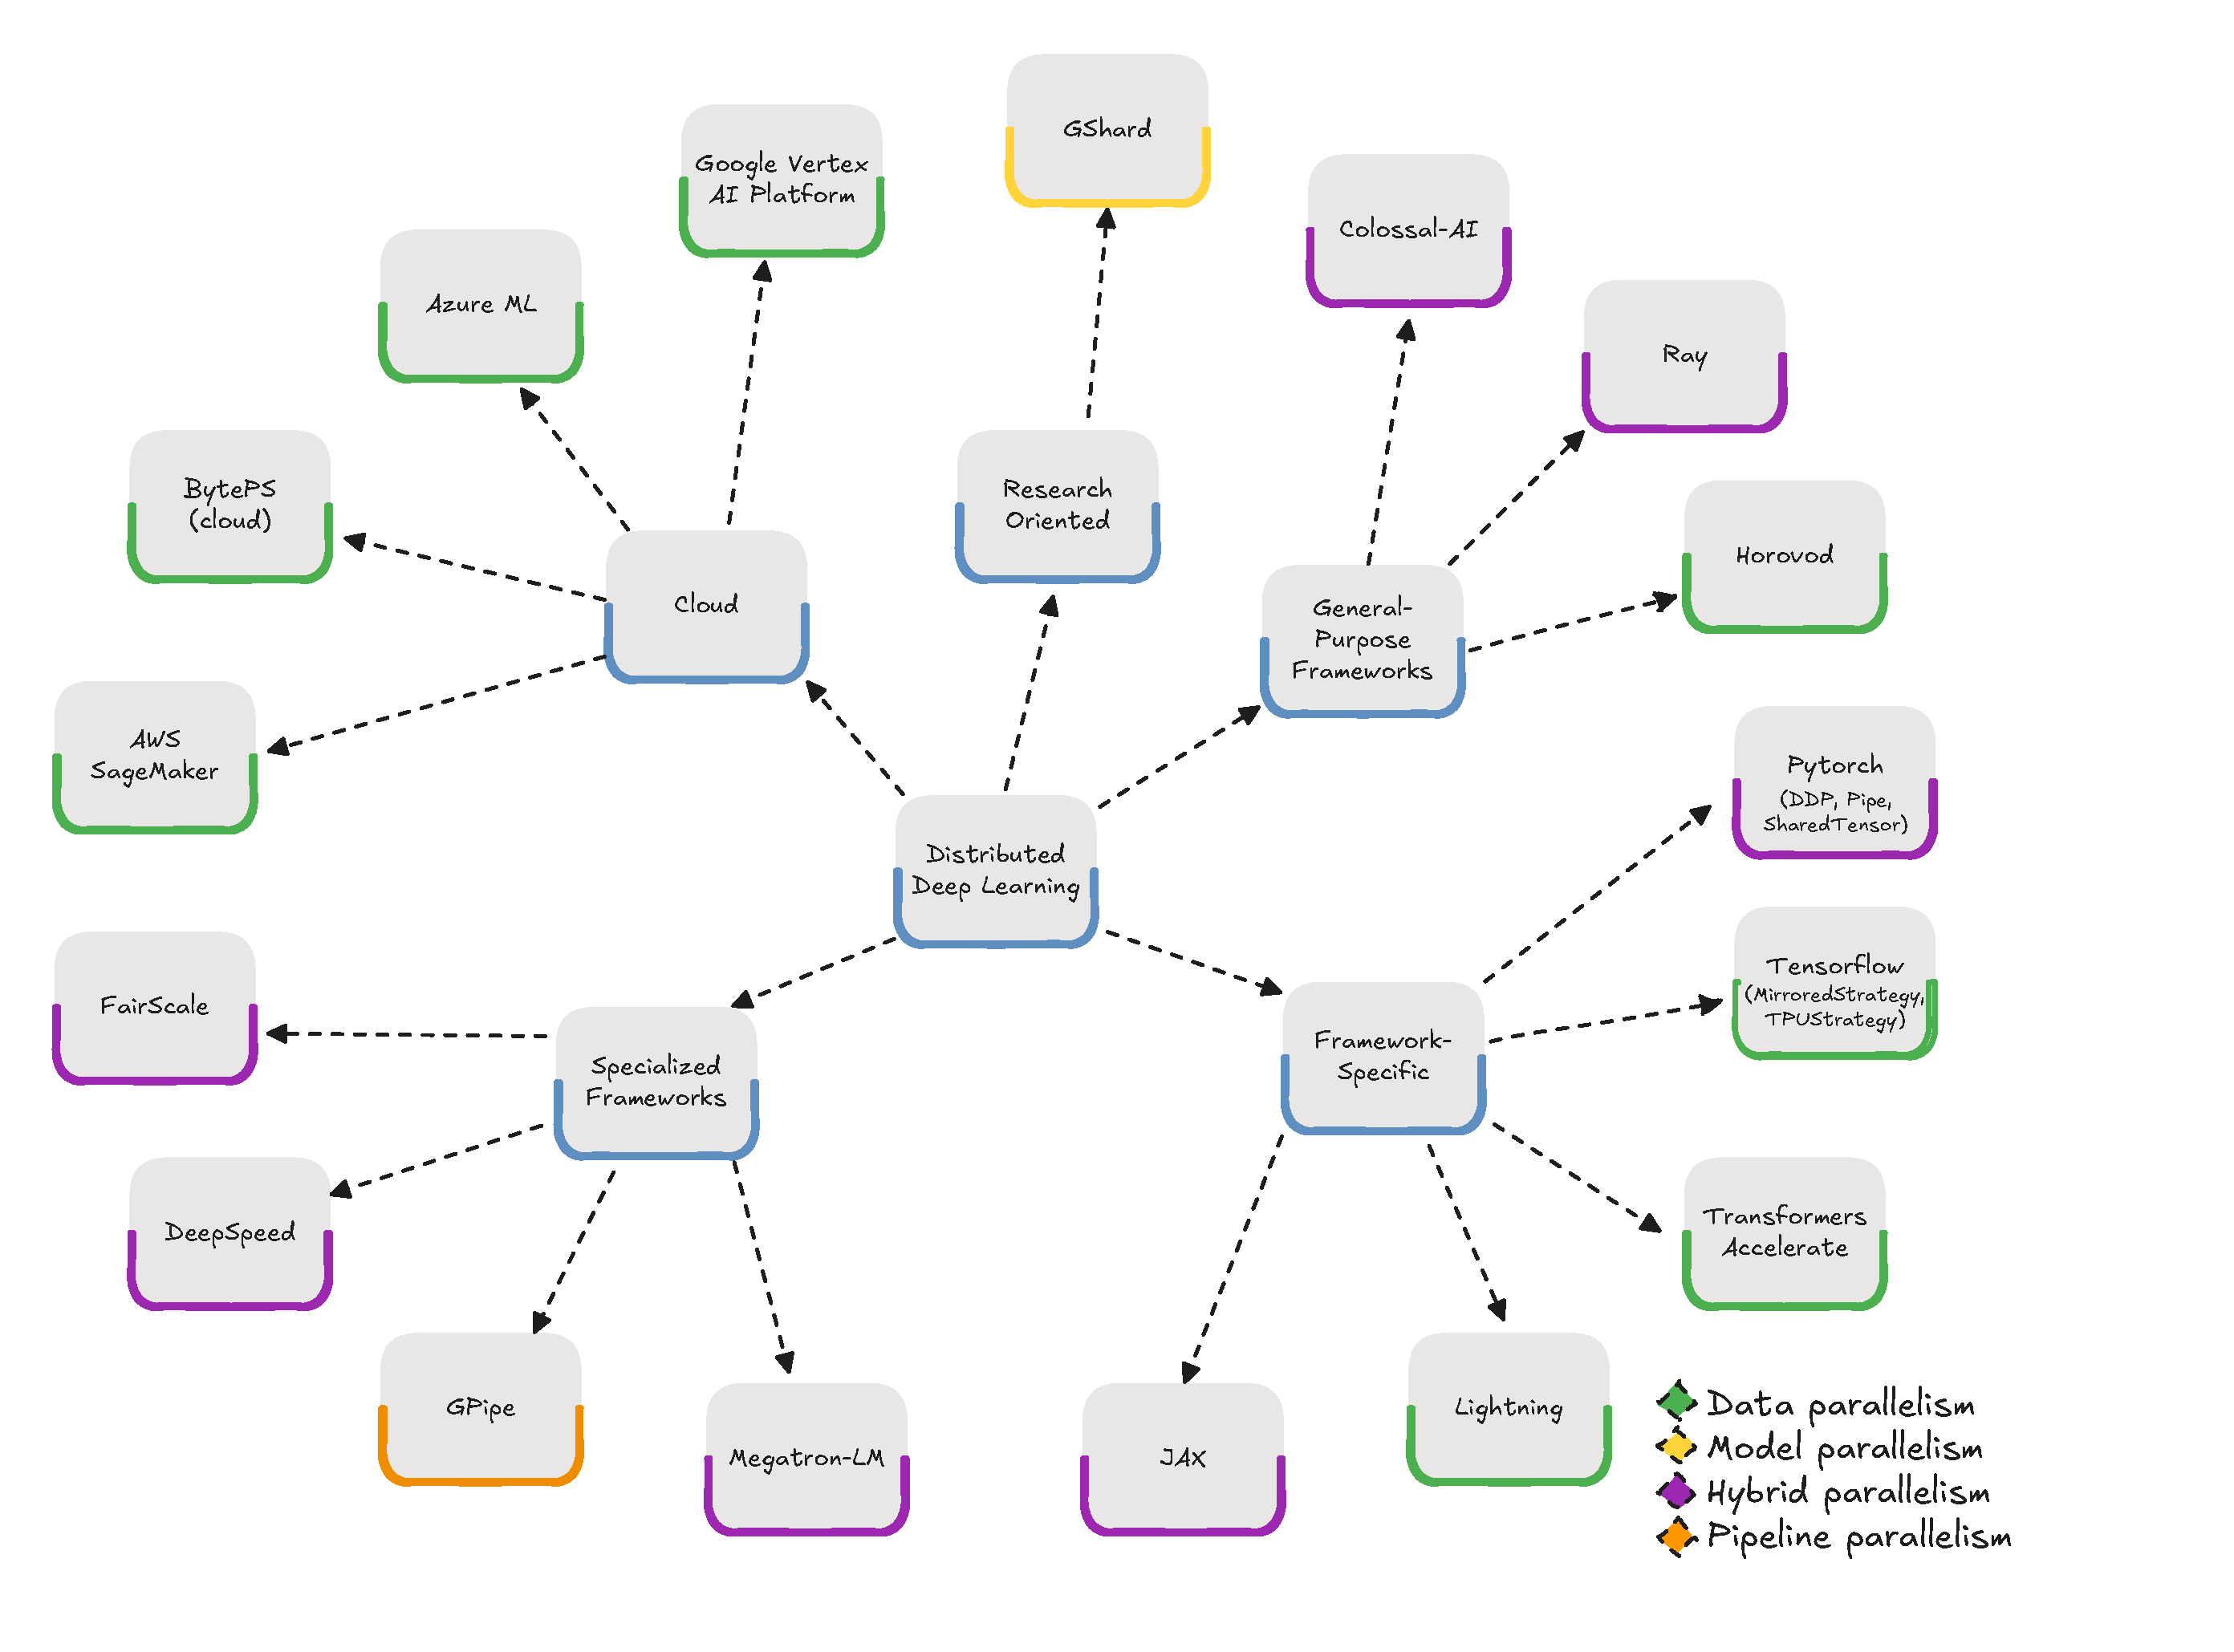
\includegraphics[width=\linewidth]{figures/mindmap}
	\caption{Mindmap.}
	\label{fig:mindmap}
\end{figure*}

\begin{figure*}[th]
	\centering
	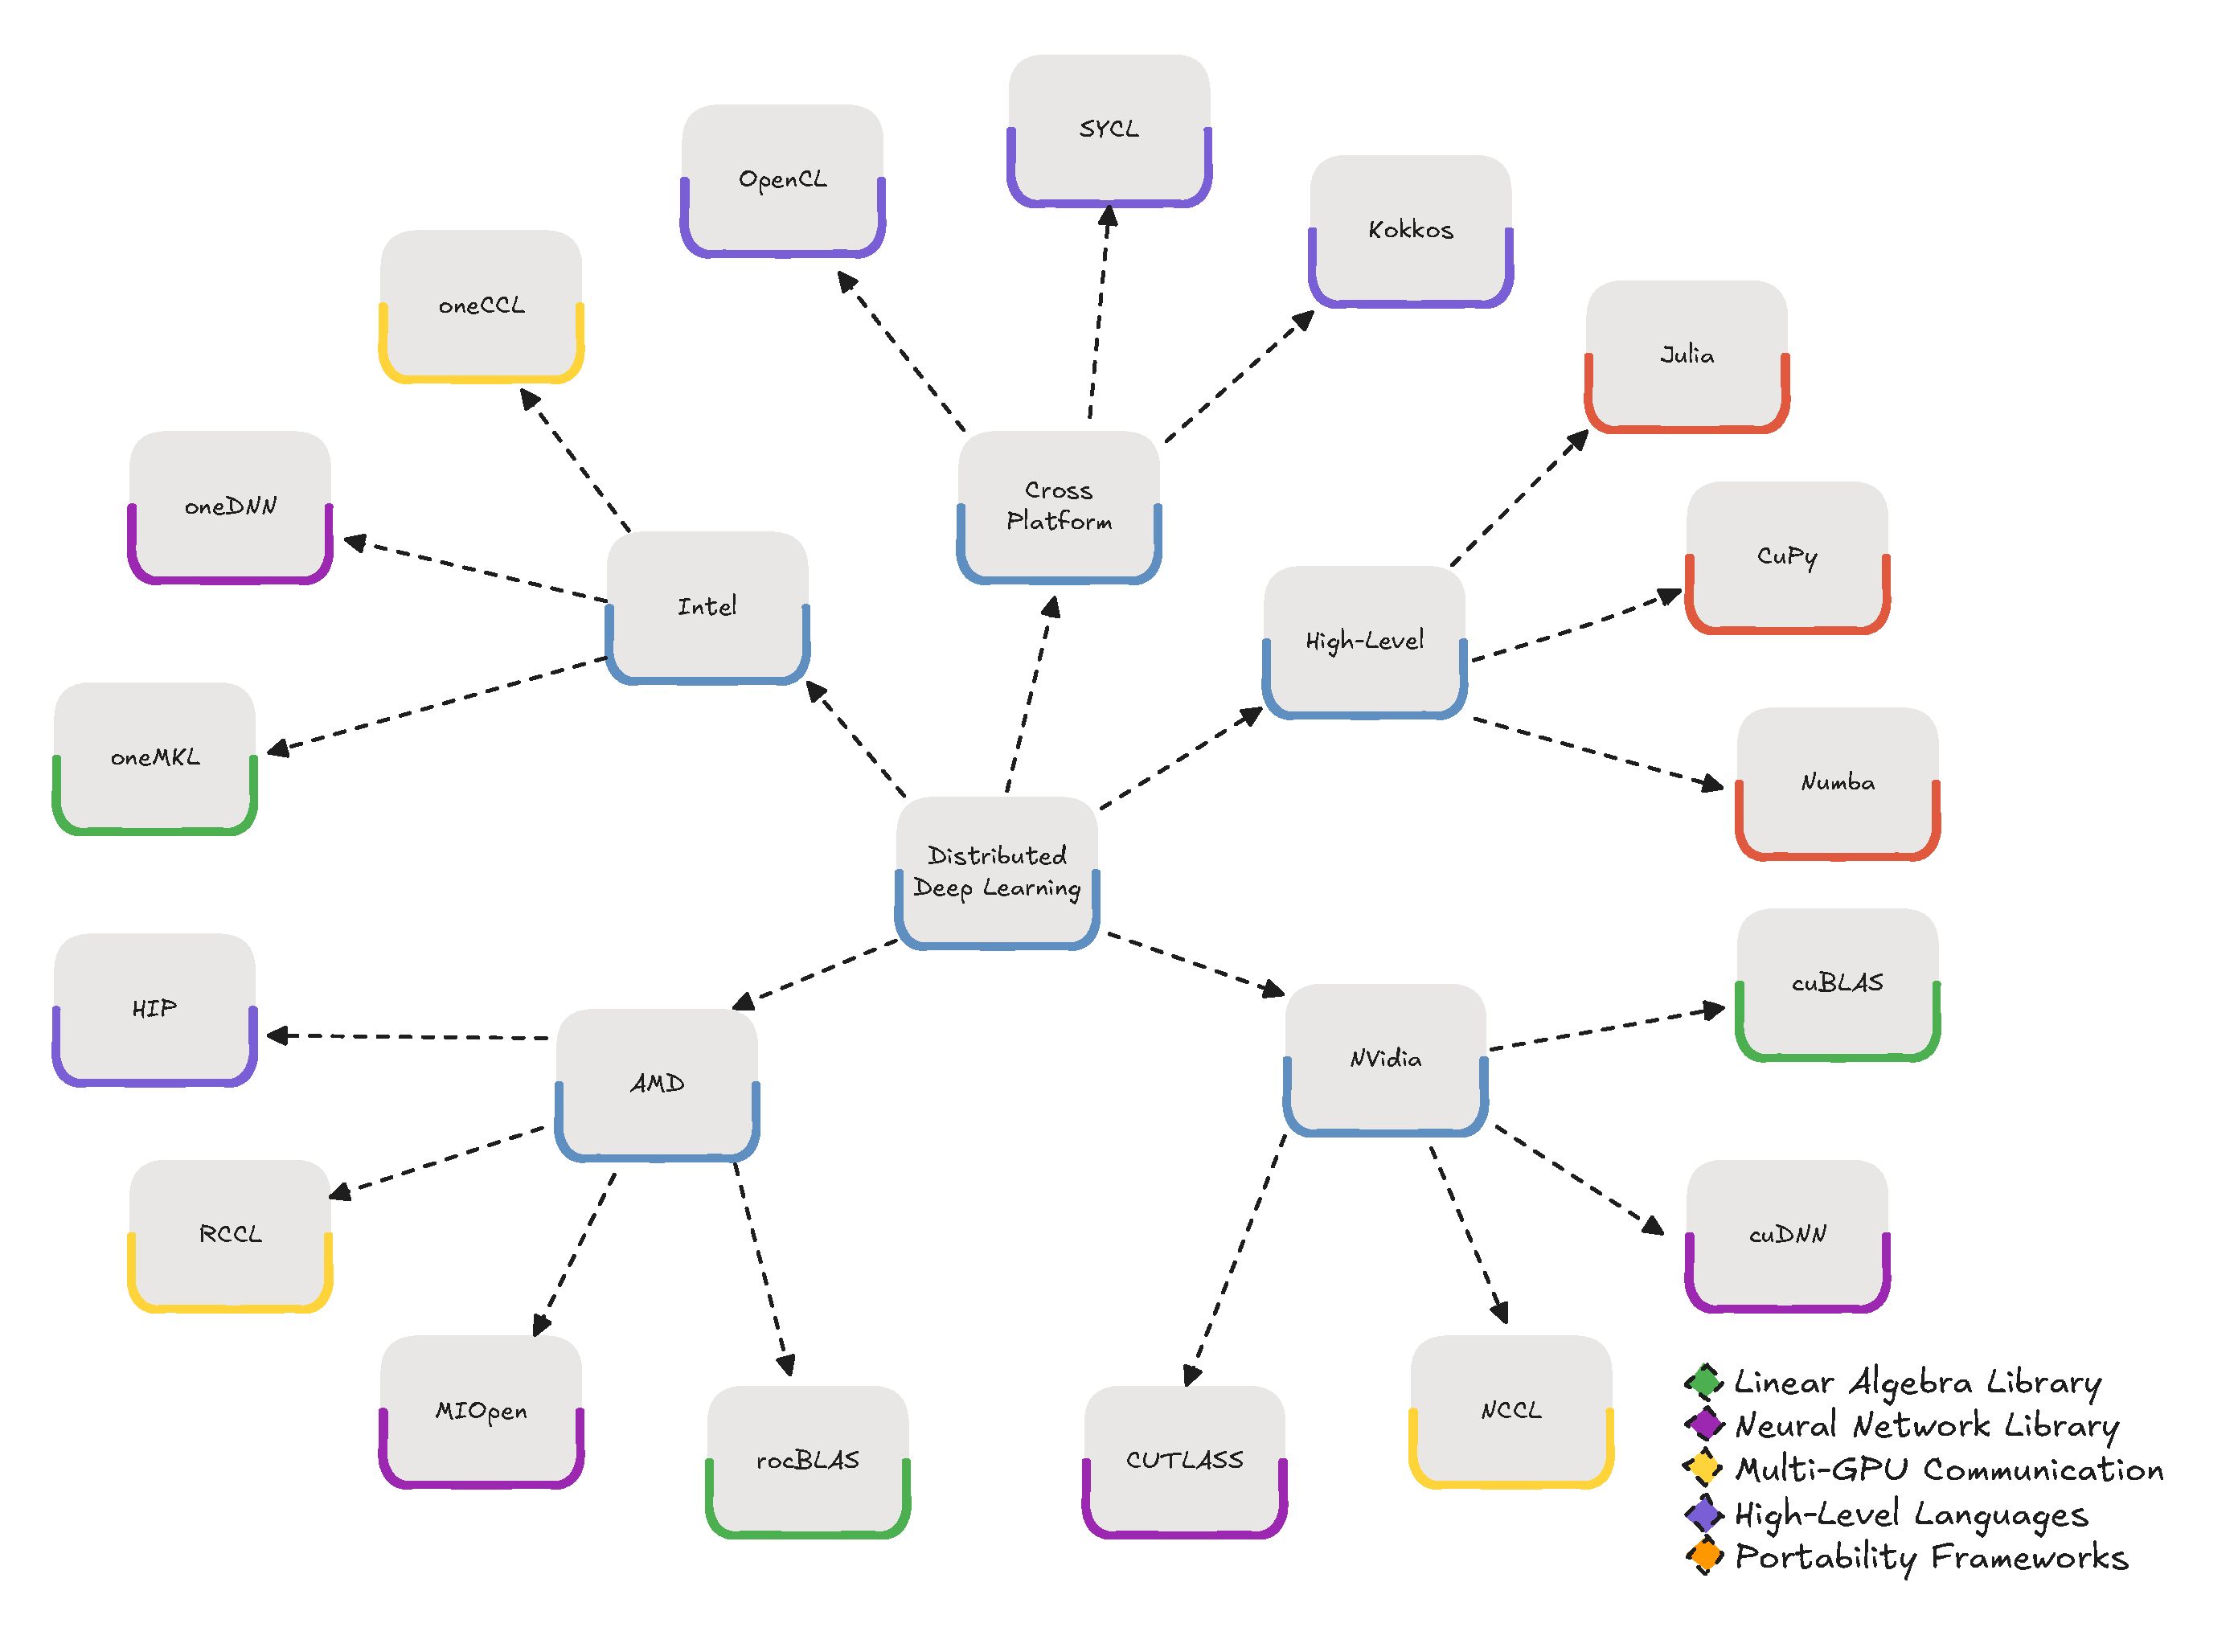
\includegraphics[width=\linewidth]{figures/mindmap-cuda}
	\caption{Mindmap.}
	\label{fig:mindmap-cuda}
\end{figure*}

% \begin{table*}[htbp]
% 	\centering
% 	\caption{The DNN papers included in the review}
% 	\label{tab2:dnn_papers}
% 	\begin{tabular}{llp{8.01cm}p{2cm}lll}
% 		\hline
% 		\textbf{\#} & \textbf{Ref.}           & \textbf{Title}                                                                & \textbf{Type} & \textbf{Year} & \textbf{Citations} & \textbf{Stars}                             \\
% 		\hline
% 		%1           & \cite{huang_gpipe_2019} & GPipe: Efficient Training of Giant Neural Networks using Pipeline Parallelism & Pipeline      & 2018          & 1446               & 2.8k \cite{noauthor_tensorflowlingvo_2025} \\
% 		2           & \cite{chen_mxnet_2015}  & MXNet: A Flexible and Efficient Machine Learning Library for Heterogeneous Distributed Systems & Hybrid (Data, Model) & 2015 & 2212 & 20.8k \cite{noauthor_apachemxnet_2025} \\
% 		% 3           & \cite{li_pytorch_2020}  & PyTorch Distributed: Experiences on Accelerating Data Parallel Training & Data & 2020 & 175 & 86.1k \cite{noauthor_pytorchpytorch_nodate} \\
% 		% 4           & \cite{abadi_tensorflow_2016} & TensorFlow: Large-Scale Machine Learning on Heterogeneous Distributed Systems & Data & 2016 & 9998 & 187k \cite{abadi_tensorflow_2015} \\
% 		% 5           & \cite{rasley_deepspeed_2020} & DeepSpeed: System Optimizations Enable Training Deep Learning Models with Over 100 Billion Parameters & Hybrid (Data, Model) & 2020 & 1059 & 36.3k \cite{noauthor_microsoftdeepspeed_2025} \\
% 		% 6           & \cite{sergeev_horovod_2018} & Horovod: fast and easy distributed deep learning in TensorFlow & Data & 2018 & 1152 & 14.3k \cite{noauthor_horovodhorovod_2025} \\
% 		% 7           & \cite{jiang_unified_nodate} & A Unified Architecture for Accelerating Distributed DNN Training in Heterogeneous GPU/CPU Clusters & Data & 2020 & 10 & 3.7k \cite{noauthor_bytedancebyteps_2025} \\
% 		% 8           & \cite{frostig_compiling_nodate} & Compiling machine learning programs via high-level tracing & Data & 2018 & 363 & 31k \cite{noauthor_jax-mljax_2025} \\
% 		\hline
% 		% Add more papers as needed
% 	\end{tabular}
% \end{table*}

\begin{table*}[htbp]
	\centering
	\caption{Critical factors of GPU Programming Libraries and Frameworks}
	\label{tab:gpu_libraries}
	\begin{tabular}{llp{8cm}lll}
		\hline
		\small \textbf{Category} & \small \textbf{ID} & \small \textbf{Library/Framework}                                 & \small \textbf{Vendor} & \small \textbf{Type} & \small \textbf{Ref.}                                  \\
		\hline
		\multirow{4}{*}{\small NVIDIA}
		                         & \small NV1         & \small cuBLAS: GPU-accelerated BLAS library for linear algebra    & \small NVIDIA          & \small Core          & \small \cite{noauthor_cublas_nodate}                  \\[1ex]
		                         & \small NV2         & \small cuDNN: Optimized deep neural network primitives            & \small NVIDIA          & \small Core          & \small \cite{chetlur_cudnn_2014}                      \\[1ex]
		                         & \small NV4         & \small NCCL: Multi-GPU/multi-node communication                   & \small NVIDIA          & \small Core          & \small \cite{noauthor_nvidianccl_2025}                \\[1ex]
		                         & \small NV5         & \small CUTLASS: Optimized C++ templates for matrix multiplication & \small NVIDIA          & \small Core          & \small \cite{thakkar_cutlass_2023}                    \\
		\hline
		\multirow{4}{*}{\small AMD}
		                         & \small AMD1        & \small rocBLAS: AMD's BLAS implementation                         & \small AMD             & \small Core          & \small \cite{noauthor_rocmrocblas_2025}               \\[1ex]
		                         & \small AMD3        & \small MIOpen: Deep learning primitives                           & \small AMD             & \small Core          & \small \cite{noauthor_rocmmiopen_2025}                \\[1ex]
		                         & \small CP4         & \small HIP: Portable API for CUDA-like code                       & \small Multiple        & \small Framework     & \small \cite{noauthor_rocmhip_2025}                   \\[1ex]
		                         & \small AMD4        & \small RCCL: Multi-GPU communication                              & \small AMD             & \small Core          & \small \cite{noauthor_rocmrccl_2025}                  \\
		\hline
		\multirow{3}{*}{\small Intel}
		                         & \small INT1        & \small oneMKL: Math Kernel Library                                & \small Intel           & \small Core          & \small \cite{noauthor_uxlfoundationonemath_2025}      \\[1ex]
		                         & \small INT2        & \small oneDNN: Deep learning primitives                           & \small Intel           & \small Core          & \small \cite{onednn_contributors_oneapi_2025}         \\[1ex]
		                         & \small INT3        & \small oneCCL: Collective communication library                   & \small Intel           & \small Core          & \small \cite{noauthor_uxlfoundationoneccl_2025}       \\
		\hline
		\multirow{3}{*}{\small Cross-Platform}
		                         & \small CP1         & \small OpenCL: Open standard for heterogeneous computing          & \small Multiple        & \small Framework     & \small \cite{noauthor_khronosgroupopencl-sdk_2025}    \\[1ex]
		                         & \small CP2         & \small SYCL: C++-based multi-device programming                   & \small Multiple        & \small Framework     & \small \cite{noauthor_khronosgroupsycl-docs_2025}     \\[1ex]
		                         & \small CP3         & \small Kokkos: Performance-portable C++ framework                 & \small Multiple        & \small Framework     & \small \cite{trott_kokkos_2022}                       \\

		\hline
		\multirow{5}{*}{\small High-Level}
		                         & \small HL1         & \small CUDA.jl: Julia GPU package for NVIDIA                      & \small NVIDIA          & \small Language      & \small \cite{noauthor_juliagpucudajl_2025}            \\[1ex]
		                         & \small HL2         & \small AMDGPU.jl: Julia GPU package for AMD                       & \small AMD             & \small Language      & \small \cite{noauthor_juliagpuamdgpujl_2025}          \\[1ex]
		                         & \small HL3         & \small oneAPI.jl: Julia GPU package for Intel                     & \small Intel           & \small Language      & \small \cite{besard_oneapijl_2022}                    \\[1ex]
		                         & \small HL4         & \small CuPy: NumPy-compatible GPU arrays for NVIDIA/AMD           & \small Multiple        & \small Language      & \small \cite{okuta_cupy_2017, noauthor_cupycupy_2025} \\[1ex]
		                         & \small HL5         & \small Numba: JIT compiler for GPU acceleration (NVIDIA only)     & \small NVIDIA          & \small Language      & \small \cite{noauthor_numbanumba_2025}                \\
		\hline
		\multirow{5}{*}{\small Tutorials}
		                         & \small T1          & \small CUDA Toolkit Samples                                       & \small NVIDIA          & \small Tutorial      & \small \cite{noauthor_nvidiacuda-samples_2025}        \\[1ex]
		                         & \small T2          & \small AMD Lab Notes                                              & \small AMD             & \small Tutorial      & \small \cite{noauthor_amdamd-lab-notes_2025}          \\[1ex]
		                         & \small T3          & \small Intel Compute Samples                                      & \small Intel           & \small Tutorial      & \small \cite{noauthor_intelcompute-samples_2025}      \\
		\hline
	\end{tabular}
\end{table*}